%
% SecMovirad: MoViRad section
%

\subsection{Background: FMCW}
\label{sec:fmcw}
During an FMCW transmission, the transmitted waveform, as shown in Fig.~\ref{fig:fmcw}, sweeps its carrier frequency linearly with respect to time between $f_{min}$ and $f_{max}$, resulting in a chirp signal being output. 

%
\begin{figure}[!htbp]
	\centering
	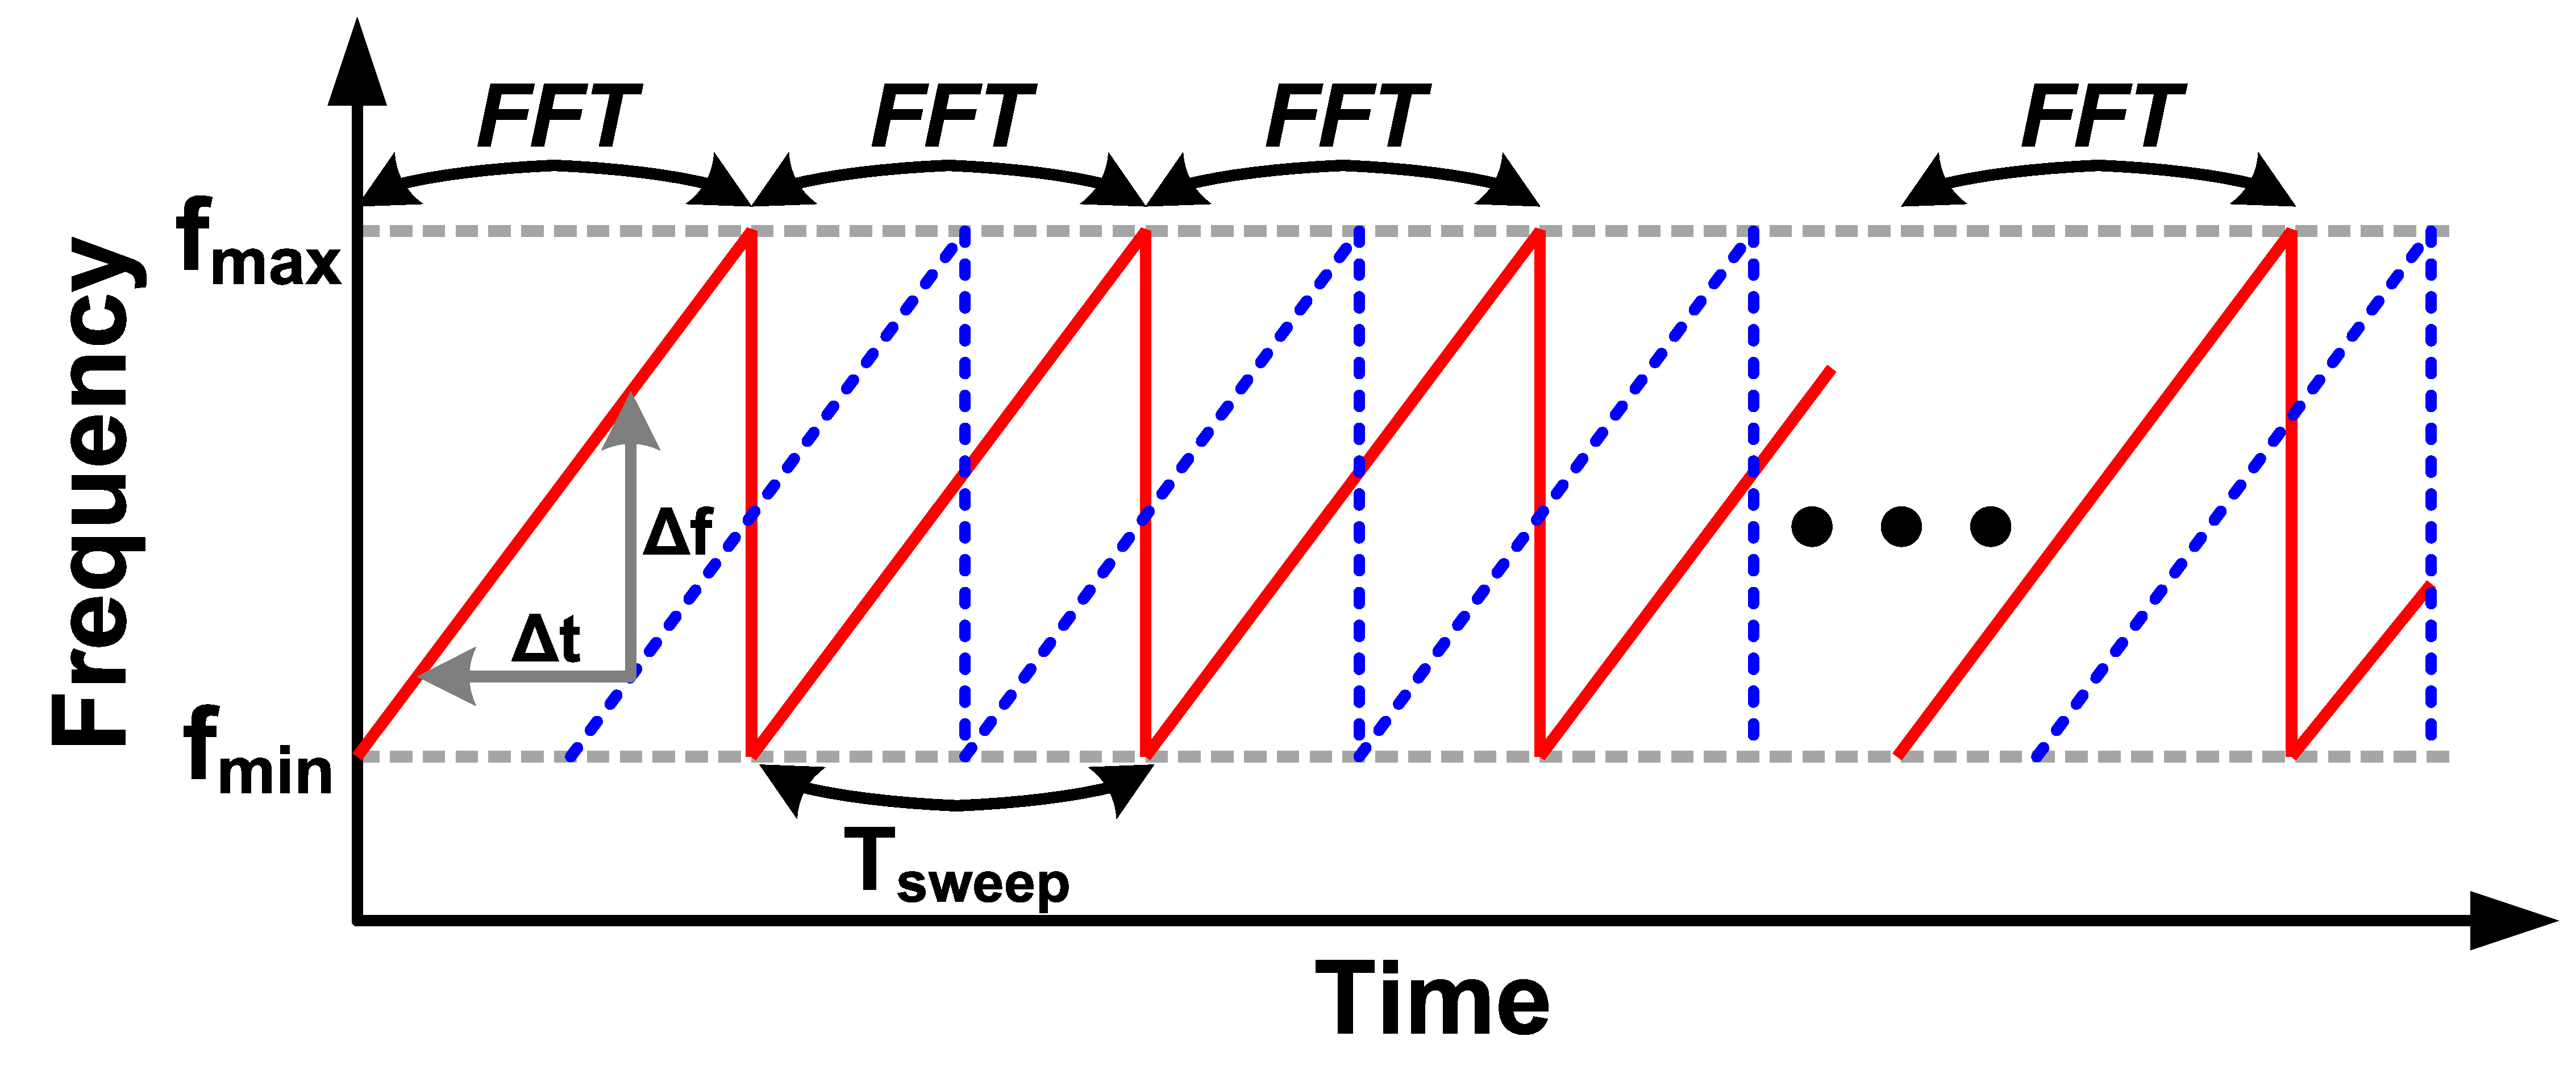
\includegraphics[width=0.9\columnwidth]{Fig01_fmcw}
	\captionsetup{justification=raggedright, singlelinecheck=false}
	\caption{Illustration of FMCW waveform.}
	\label{fig:fmcw}
\end{figure}
%

As shown in Fig.~\ref{fig:fmcw}, for instance, the red line represents the transmitted signal and the blue line represents received signal. The time delay, labeled as $\Delta t$ in the figure, is proportional related to the slope of the linear sweeping segment of the chirp. In other words, the frequency shift between transmitted and received signal could be accurately extracted from the transmission delay. Denoting the sweeping period of the chirp as $T_{sweep}$, the frequency offset $\Delta f$ can be calculated as:

%
\begin{equation}
	\label{eqn:fmcw_df}
	\Delta f = \dfrac{f_{max} - f_{min}}{T_{sweep}} \cdot \Delta t
\end{equation}
%

and the delay could be measured as:

%
\begin{equation}
	\label{eqn:fmcw_dt}
	\Delta t = \dfrac{2 \cdot d}{v_{wave}}
\end{equation}
%

where $d$ denotes the distance between transmitter and the object under test, and $\rm v_{wave}$ is the propagation velocity of the wave.

Consequently, in order to measure minute distance change such as breathing, we could send a signal towards the person so that we could back calculate the periodic chest movement associated with the breathing. Similar to the processing demonstrated in~\cite{Adib_acm15,nandakumar_mobisys15}, we apply FFT on the received signal and the perform peak search for the breathing signal. Assuming that acoustic wave travels at speed of 340m/sec at room temperature, the accuracy that we are able to achieve is roughly 2cm given that the mobile phone's microphone has a sampling rate of 44.1kHz.

\subsection{FFT Interpolation}
\label{sec:fftinterp}
While 2cm resolution is adequate for breathing, we are not able to recover heart beat signal which may only cause the chest to move in the order of millimeter. Hence, we proposed a novel interpolation method on the FFT peak search to improve the achievable accuracy. The interpolation of FFT peak is performed as follows:

%
\begin{enumerate}
	\item Perform a peak search in the correct "bucket" given a pre-knowledge of the estimated frequency, and assume only one peak resides in the frequency range of interest.
	\item Since the peak is very unlikely to fall exactly in one bin, we interpolate the peak and the second largest value to find a precise phase offset using the FFT. Interpolation revolves around the two consecutive FFT samples based on the initial peak search result. Denote the peak index with $\rm k$, and the next highest peak index with $\rm k + 1$. By taking the ratio of two consecutive samples, we wil find a ratio $\rm R$:
	
	%
	\begin{equation}
		\label{eqn:ratio}
		R = \dfrac{X[k]}{X[k+1]} = \dfrac{1 - r e^{-\frac{j2\pi}{N}}}{1 -r}
	\end{equation}
	%

	where $\rm r = e^{\frac{j2\pi\delta}{N}}$ is the frequency shift, and $\rm \delta$ is our fine frequency offset. In other words, we can now solve for $r$ now as a function of $R$, and extract the phase information from that.
	\item Use the previously mentioned coarse tracking plus the additional fine tracking to get precise distance measurements
\end{enumerate} 
%

It is worth notice that the proposed interpolation method revolves around the definition of the FFT, and the fine resolution is guaranteed with appropriately selected sweep frequency ($f_{min}$ and $f_{max}$) of the chirp signal. For this project, we sweep the signal from 10kHz to 20kHz with a sweep time of 50ms, targeting a maximum distance of 2m, we can achieve a distance measurement with a maximum error of 0.25mm. Also, this method could be applied to identify multiple people simultaneously if they are separated sufficiently for our course FFT to resolve ($>$2cm). In presence of three signals, assuming each 5cm apart distance, we are able to extract three distinct peak from the received signals while still maintaining a maximum error of 7.2mm.

For the above analysis, we have assumed that only one peak reside in the frequency spectrum of interest. However, in practice, it may occur that multiple peaks of comparative power are identified within the same frequency range. Under such condition, our coarse FFT cannot resolve them individually, resulting in large errors for further analysis. For this project, we will be focusing on demonstrating the feasiblity of implementing Vital-Radio idea~\cite{Adib_acm15} using mobile phone. So the testing is conducted to ensure only one moving object at presence.





